\chapter{To verify the truth table for AND Gate}
%\ref{sec:background}.

%\section{Aim}
%\label{sec:objectives}
%	To verify the truth table for AND Gate.

\section{Apparatus}
%\label{sec:objectives}
	\begin{itemize}
		\tightlist
		\item Kit for realization of gates
		\item Connecting Leads
	\end{itemize}

\section{Theory}
	The AND gate is an electronic circuit that gives a high output (1) only if all its inputs are high. A dot (.) is used to show the AND operation i.e. A.B or can be written as AB
	\begin{figure}[h]
		\centering
		
\includegraphics{img/exp1/1}
		\caption{Symbol for AND gate}
		\label{fig:and_gate}
	\end{figure}
	\begin{figure}[h]
		\centering
		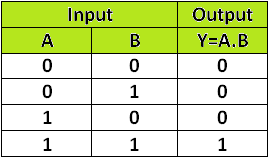
\includegraphics{img/exp1/2}
		\caption{Truth Table for AND gate}
		\label{fig:and_gate_table}
	\end{figure}
	A simple 2-input logic AND gate can be constructed using RTL (Resistor-Transistor-Logic) switches connected together as shown below with the inputs connected directly to the transistor bases. Both transistors must be saturated “ON” for an output at Q.
	
	\begin{figure}[h]
		\centering
		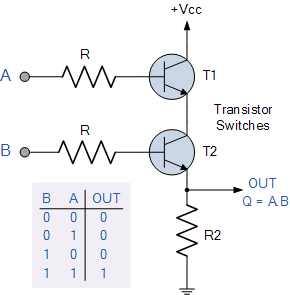
\includegraphics{img/exp1/3}
		\caption{Circut for making AND gate}
		\label{fig:and_diag}
	\end{figure}
	
	

		
\section{Procedure}
	\subsubsection{Simulator 1}
	\begin{itemize}
		\tightlist
		\item Connect the supply(+5V) to the circuit.
		\item Press the switches for inputs "A" and "B".
		\item The bulb does not glow if any one or both the switches (2 and 3) are OFF and glows only if both the switches (2 and 3) are ON.
		\item Repeat step-2 and step-3 for all state of inputs.
	\end{itemize}

	\subsubsection{Simulator 2}
	\begin{itemize}
		\tightlist
		\item Enter the Boolean input "A" and "B".
		\item Enter the Boolean output for your corresponding inputs.
		\item Click on "Check" Button to verify your output.
		\item Click "Print" if you want to get print out of Truth Table.
	\end{itemize}


\section{Observations}
	\begin{figure}[h]
		\centering
		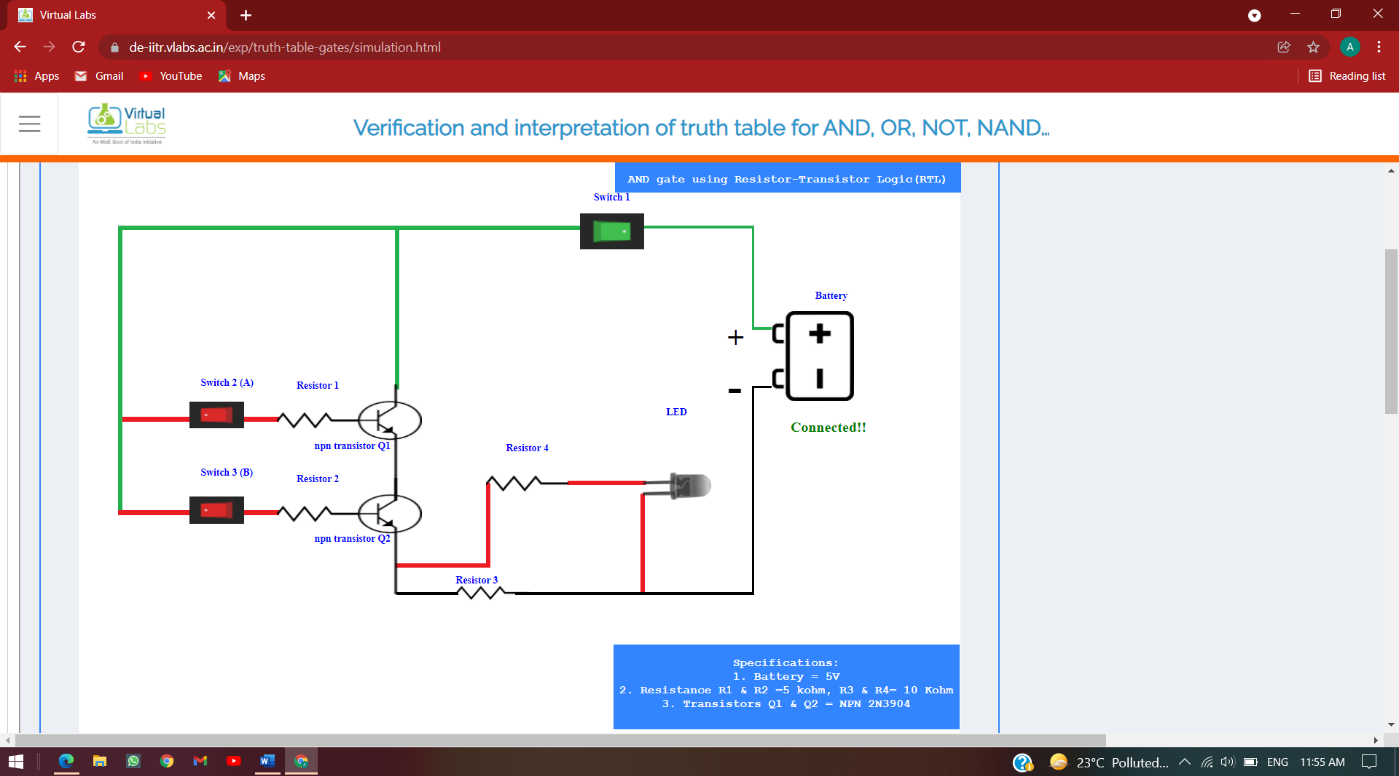
\includegraphics[width=0.9\linewidth]{img/exp1/4}
		\caption{}
		\label{fig:1:4}
	\end{figure}
		\begin{figure}[h]
		\centering
		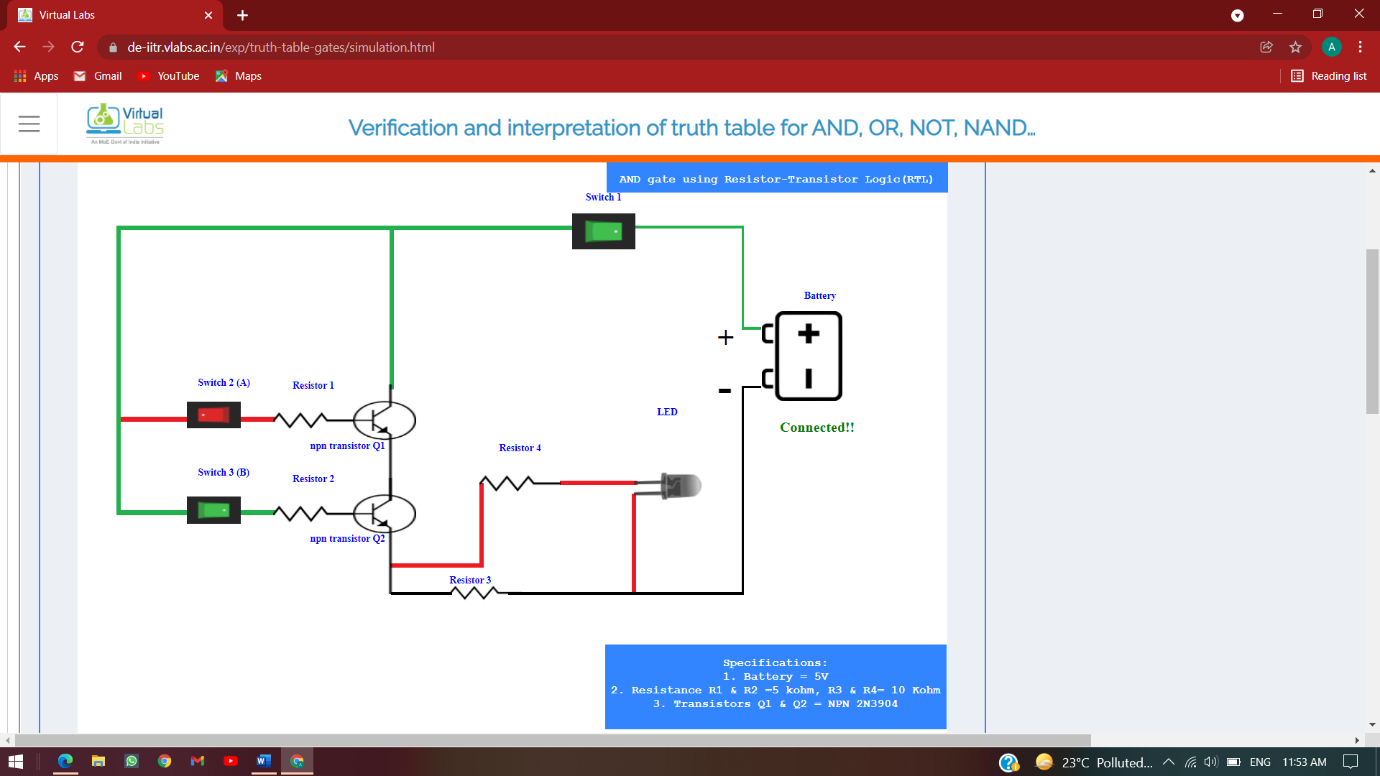
\includegraphics[width=0.9\linewidth]{img/exp1/5}
		\caption{}
		\label{fig:1:5}
	\end{figure}
		\begin{figure}[h]
		\centering
		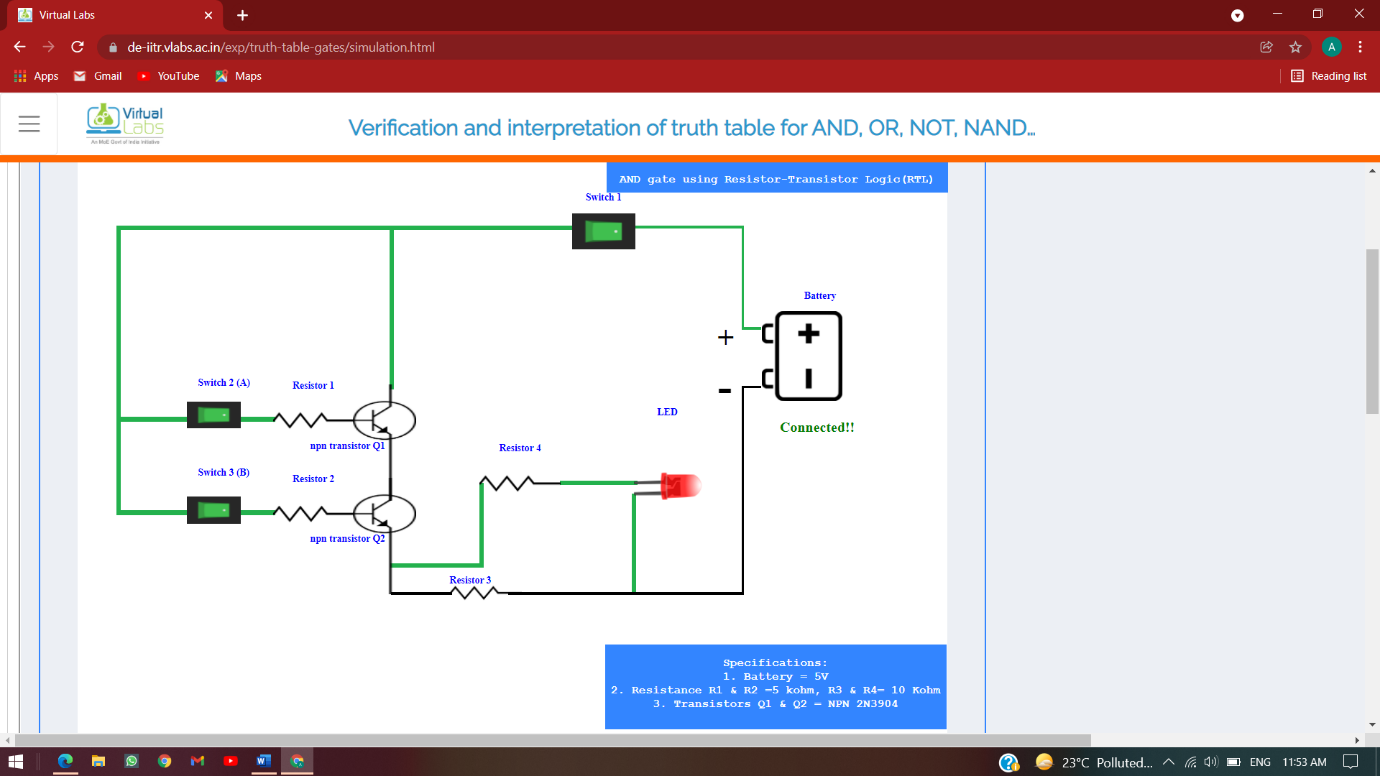
\includegraphics[width=0.9\linewidth]{img/exp1/6}
		\caption{}
		\label{fig:1:6}
	\end{figure}
		\begin{figure}[h]
		\centering
		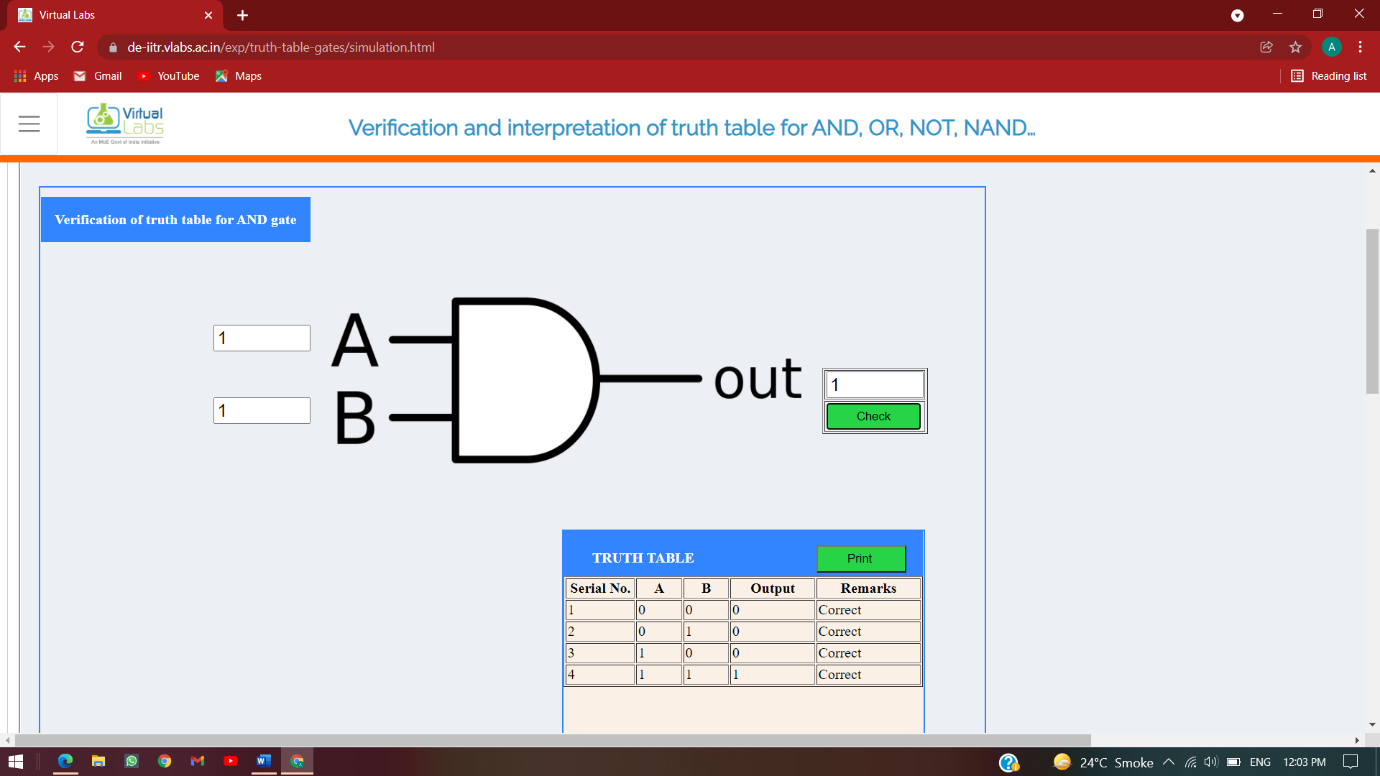
\includegraphics[width=0.9\linewidth]{img/exp1/7}
		\caption{}
		\label{fig:1:7}
	\end{figure}

\section{Conclusion}
Thus we can conclude that if both inputs are high then only the output is high but if even one of the inputs is low the output is low.

\section{Precautions}
	\begin{enumerate}
		\tightlist
		\item Make the connections when power supply is OFF.
		\item Ensure that the connections are tight.
		\item Change the status of inputs only when power supply is OFF.
	\end{enumerate}